\documentclass[12pt]{exam}
\newcommand{\hwnumber}{6}
\newcommand{\hwname}{Text Buffers}
\newcommand{\duedate}{\formatdate{7}{03}{\YEAR} by \progDueTime}

\usepackage{../misc/latex/edition}  % Course semester
\usepackage{../misc/latex/c0}       % Listings style for c0
\usepackage{amsmath}
\usepackage{enumerate}
\usepackage[normalem]{ulem}
\usepackage{verbatim}
\usepackage[left=1in, right=1in, top=1in, bottom=1in]{geometry}
\usepackage{graphicx}
\usepackage{hyperref}
\usepackage{tikz}     \usetikzlibrary{shapes}
\usepackage{fancybox}
\usepackage[all]{xy}
\usepackage{wrapfig}
\usepackage{fancyvrb}
\usepackage{datetime}
\usepackage{etoolbox}
\usepackage{calc}
\usepackage[nomessages]{fp}
\usepackage{import}  % Like input and include, but respects subdirectories

\newcommand{\defaultQuestionLocation}{questions}
\newcommand{\inputQuestion}[2][\defaultQuestionLocation/]{%
  \subimport{#1}{#2}
}
% Subdirectories of \defaultQuestionLocation containing code and pictures
\newcommand{\code}{code}
\newcommand{\img}{img}


%%% ic: frontmatter macros
\newcommand{\specialInstructions}{}
\newcommand{\HWNUMBER}
{\ifdefempty{\hwnumber}{__}{%
  \ifnumless{\hwnumber}{10}{0\hwnumber}{\hwnumber}}}
\newcommand{\hwtype}{Written Homework}

%%% ic: 'exam' tweaks
\renewcommand{\half}{.5} % Half points

\newcommand{\Question}[2][]
 {\ifstrempty{#1}
    {\question{\bf #2}}
    {\question[#1]{\bf #2}}
  \immediate\write\rubricfile{}%
  \immediate\write\rubricfile{Question \thequestiontitle:}%
  \immediate\write\rubricfile{==========}
 }

%%% ic: Support for editable PDF
% counter name (some viewers misbehave if always the same)
\newcounter{editable}
\newcommand{\nextField}{\addtocounter{editable}{1}q\arabic{editable}}
\newcommand{\NextField}
 {\makebox[0pt][r]{\scalebox{0.1}{\color{White}\nextField}}}

% Color of edit area
\newcommand{\editAreaColor}{red}
% Single line answer:   \editableLine[extra parameters (optional)]{line width}
\newcommand{\editableLine}[2][]
{\textcolor{\editAreaColor}{%
 \underline{\hspace*{-0.25em}%
 \raisebox{-0.5ex}{%
 \TextField[width=#2, borderwidth=0, #1]{\NextField}}}}%
}
% Single line answer for code:  \editableLine[extra parameters (optional)]{line width}
\newcommand{\editableCodeLine}[2][]
{\textcolor{\editAreaColor}{%
 \underline{%
 \TextField[width=#2, height=1.5ex, borderwidth=0, #1]{\NextField}}}}
% Multiline answer:  \editableLine[extra parameters (optional)]{box height}
\newcommand{\editableBox}[2][]
{\leavevmode\hspace*{-0.1em}%
\TextField[height=#2, width=\linewidth,
           multiline=true, borderwidth=0.1, bordercolor=\editAreaColor,
           #1]{\NextField}}

%%%%% Same answer format as exams
\renewcommand{\rmdefault}{ppl}
\renewcommand{\sfdefault}{phv}
\newcommand{\answerColor}{Blue}

\ifprintanswers
\newcommand{\answer}[2]{\makebox[#1][c]{\color{\answerColor}#2}}
\else
\newcommand{\answer}[2]{\makebox[#1][c]{}\makebox[0pt]{\phantom{|}}}
\fi
\newcommand{\uanswer}[2]{\underline{\answer{#1}{#2}}}


%%% Write rubric snippet.  Usage:
% \RUBRIC
% any multi-line text (including \, #, %, whatever)
% ENDRUBRIC
%% (ENDRUBRIC should be on a line by itself)
\makeatletter
\def\RUBRIC
 {%
  \begingroup
  \let\do\@makeother\dospecials
  \endlinechar=`\^^J
  \@tofile%
 }
\def\ENDRUBRIC{ENDRUBRIC}
\def\@tofile#1^^J{%
  \def\@test{#1}%
  \ifx\@test\ENDRUBRIC
    \immediate\write\rubricfile{}  % End with an empty line
    \expandafter\@firstoftwo
  \else
    \expandafter\@secondoftwo
  \fi
  {\endgroup}%
  {\toks@{#1}%
   \begingroup\endlinechar=\m@ne
   \everyeof{\noexpand}%
   \xdef\@temp{\scantokens\expandafter{\the\toks@}}%
   \endgroup
   \immediate\write\rubricfile{\@temp}%
   \@tofile}%
}
\makeatother

%% Displays tags for an exercise in 'answer' mode
\newcommand{\TAGS}[1]
{\ifprintanswers%
  \rule{0em}{0ex}%
  \marginpar{\footnotesize%
    \fcolorbox{black}{Gray!25}{%
      \parbox[t]{2cm}{\raggedright\textbf{TAGS:}\\#1}}}%
  \ignorespaces%
 \fi}%


%% Page layout
\pagestyle{headandfoot}

\headrule
\header{\textbf{\courseNumber{} \hwtype{} \hwnumber}}
       {}
       {\textbf{Page \thepage\ of \numpages}}
\footrule
\footer{}{}{\COPYRIGHT}

\renewcommand{\partlabel}{\textbf{\thequestion.\thepartno}}
%\renewcommand{\partlabel}{\textbf{Task \thepartno}}
\renewcommand{\subpartlabel}{\textbf{\thesubpart.}}
\renewcommand{\thepartno}{\arabic{partno}}
\renewcommand{\thesubpart}{\alph{subpart}}
\pointpoints{pt}{pts}
\pointformat{\raisebox{0ex}[\height][0pt]{\fcolorbox{black}{yellow}{\themarginpoints}}}
\bonuspointformat{\raisebox{0ex}[\height][0pt]{\fcolorbox{black}{red}{\themarginpoints}}}
\marginpointname{\points}
\pointsinmargin
%\boxedpoints

\setlength\answerlinelength{2in}
\setlength\answerskip{0.3in}

\newcommand{\mkWrittenTitle}[1]{#1}
\newcommand{\mkDueDate}[1]{#1}
\newcommand{\mkEvalSummary}[1]{#1}
\newcommand{\mkGradetable}[1]{#1}



% This fixes an issue with the exam package version 2.6 and after,
% where 'framed' has been renamed to 'examframed' to avoid a conflict.
\ifcsmacro{examframed}{%
\newenvironment{framed}
{\begin{examframed}}
{\end{examframed}}
}{}

\begin{document}
\hwTitle

\noindent
For the programming portion of this week's homework, you'll use a doubly
linked list to implement some of the basic features of a text editor.

\bigskip
\noindent
The code handout for this assignment is on \autolab{} and at
\begin{center}
\whereisthetgz{tbuf-handout.tgz}
\end{center}
The file \lstinline'README.txt' in the code handout goes over the contents
of the handout and explains how to hand the assignment in.
There is a SIX (6) PENALTY-FREE HANDIN LIMIT.
Every additional handin will incur a small (5\%) penalty (even if
using a late day).


\paragraph{Warning:}

In the course so far, we have previously considered interfaces (like
pixels, stacks, queues, and dictionaries) that did not expose their internal
representation to the user and that were tested as an opaque interface
(black-box testing). The data structures and interfaces we implement
for this assignment expose their internal representation to the
client.

The expectation is that the client (who is sometimes the text editor,
and sometimes you!) will mostly use this representation to read from
the data structures, but they will usually not write to the data
structures themselves.  However, clients are allowed to manipulate the
data structures, and so we expose the data structure invariants (like
\lstinline'is_tbuf') as part of the interface.

This means that your data structure invariants will need to be
\emph{very good}, and we will test them very thoroughly. They need to
permit anything permitted by the specification, and disallow anything
that is not allowed by the specification. One thing we will
\emph{not} require you to do in this assignment is circularity checking: we
will never test your data structures against a doubly linked list
where you can follow \lstinline'next' pointers forever without reaching
\lstinline'NULL' or one where you can follow \lstinline'prev' pointers forever
without reaching \lstinline'NULL'.


\clearpage
\section{Doubly linked lists with cursors}

We have seen singly-linked lists used to represent stacks and queues ---
sequences of nodes, each node containing some data and a pointer to the next
node.  The nodes in a \emph{doubly-linked list} contain instead \emph{two}
pointers: one to the next element (\lstinline'next') and one to the
\emph{previous} element (\lstinline'prev').  They have a \lstinline'data'
field just like those of a singly-linked list.

We will use doubly-linked lists to hold the contents of an editor.
An \emph{editable sequence} is represented in memory by a doubly-linked list
and two pointers: one to the \lstinline'start' of the sequence, one to
the \lstinline'end' of the sequence.  We employ our usual trick of
terminating the list (on both ends!) with ``dummy'' nodes whose
contents we never inspect.
\begin{quote}
\begin{lstlisting}[numbers=none]
typedef struct dll_node dll;
struct dll_node {
    dll* prev;
    elem data;
    dll* next;
};
\end{lstlisting}
\end{quote}
The following doubly linked list contains the text
``spaces'':
\begin{center}
  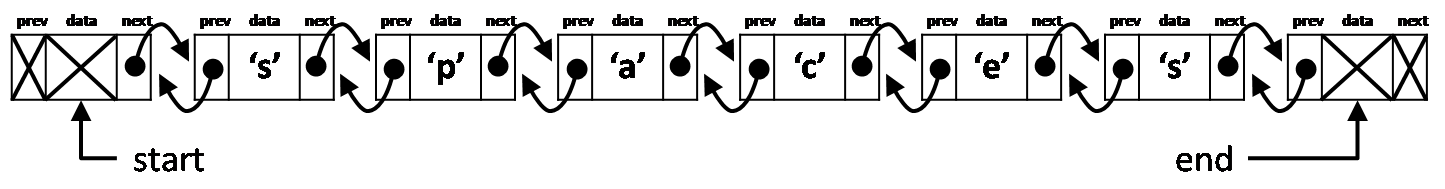
\includegraphics[width=0.95\textwidth]{\img/dll1.png}
\end{center}
To use a doubly linked list as a text buffer, we need to add a
\emph{cursor}, which represents the position where edits can be made
in the buffer. In an Emacs-like interface, the cursor frequently
appears as a black rectangle, so that if the cursor was pointing to the
node containing the character \lstinline"'e'", we'd see it displayed as
\begin{center}
\begin{tikzpicture}
\draw (0.0,0) node{\large\texttt{spaces}};
\draw [line width=8] (.405,-.3) -- (.405,.32);
\draw (0.0,0) node{\large\texttt{\color{white}spaces~~~~~~~~e~~~~~spaces}};
\end{tikzpicture}
\end{center}
Pressing the left arrow key in a text editor moves the cursor one
character backward (to the left).
\begin{center}
\begin{tikzpicture}
\draw (0.0,0) node{\large\texttt{spaces}};
\draw [line width=8] (.14,-.3) -- (.14,.32);
\draw (0.0,0) node{\large\texttt{\color{white}spaces~~~~~~~c~~~~~~spaces}};
\end{tikzpicture}
\end{center}
We can now draw the linked list corresponding to this text buffer
along with its header, which contains \lstinline'start',
\lstinline'cursor', and \lstinline'end' fields:
\begin{center}
  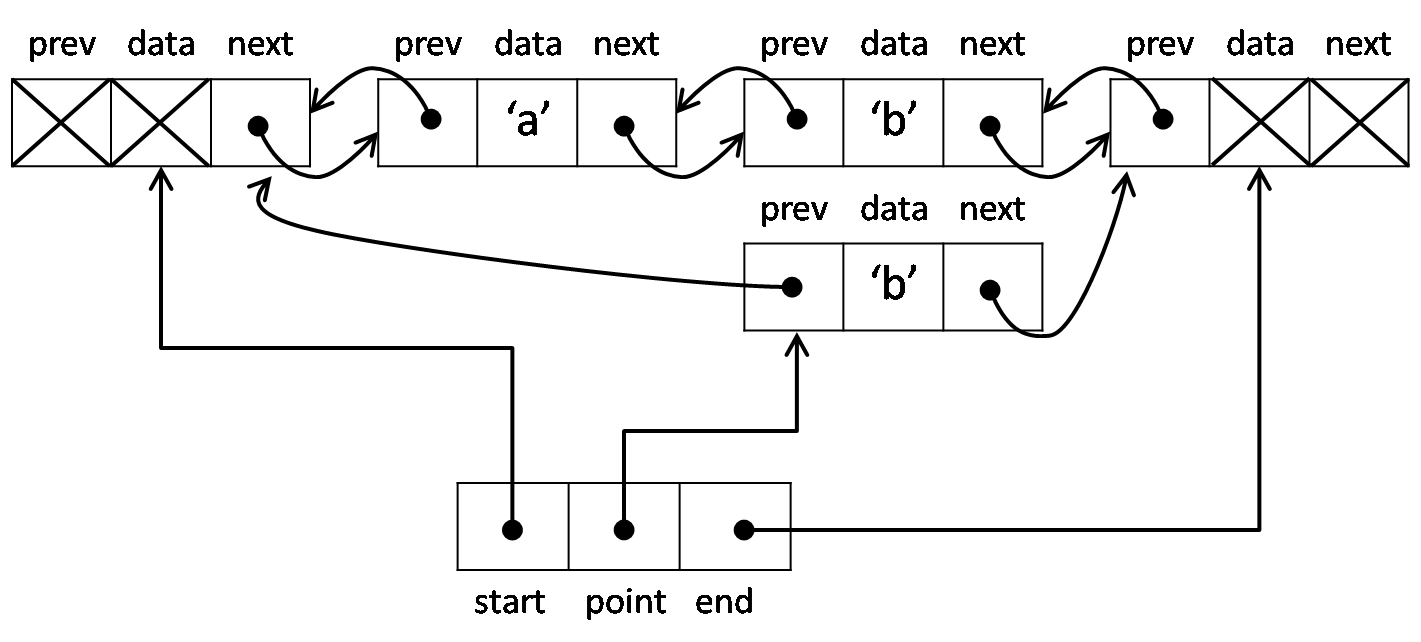
\includegraphics[width=0.95\textwidth]{\img/dll2.png}
\end{center}

\newpage
Edits in a text buffer take place to the left of the cursor. If we
press the ``delete'' key in the previous picture, it will delete the
character to the left of the cursor:
\begin{center}
  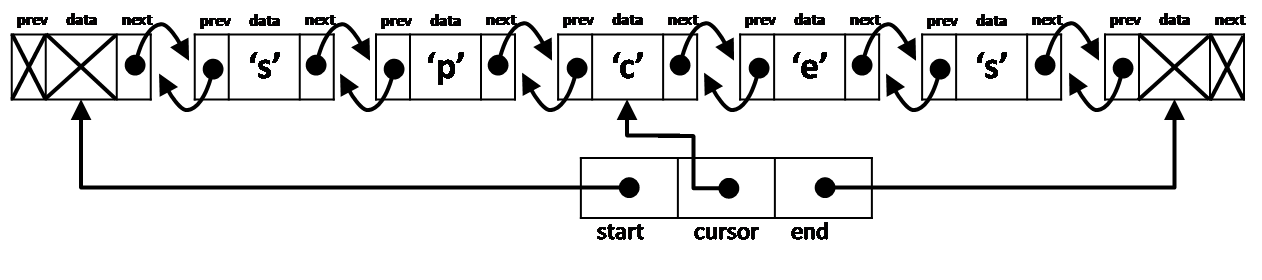
\includegraphics[width=0.95\textwidth]{\img/dll3.png}
\end{center}\vspace{-2.5ex}
Insertions also happen to the left of the cursor. If we next typed the
``i'' key, that character would be entered in to the right of the
buffer.
\begin{center}
  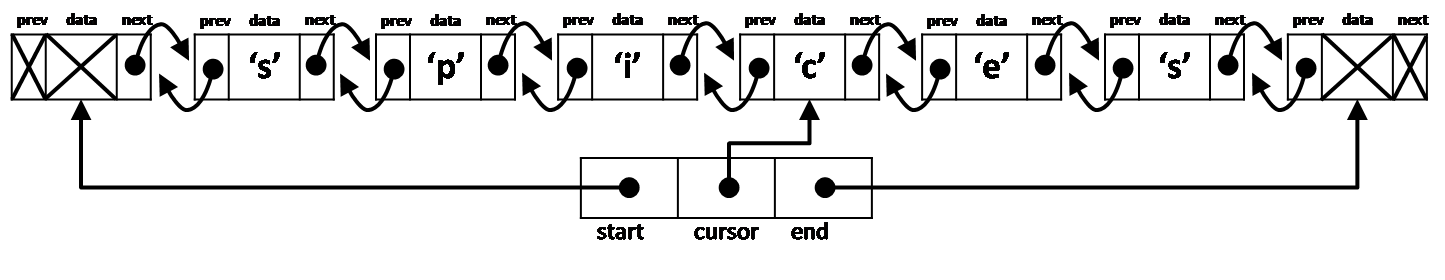
\includegraphics[width=0.95\textwidth]{\img/dll4.png}
\end{center}\vspace{-2.5ex}
One consequence of this design is that, in order for additions and
deletions to be made to the end of the buffer, the cursor needs to be
able to go to the right of all the text. In other words, it must be
possible for the \lstinline'cursor' field to point to the same node
that \lstinline'end' points to. Starting from the buffer above, we can
see what that looks like from the editor's point of view:
\begin{center}
\begin{tikzpicture}
\draw (0.0,0) node{\large\texttt{spices}};
\draw [line width=8] (.14,-.3) -- (.14,.32);
\draw (0.0,0) node{\large\texttt{\color{white}spices~~~~~~~c~~~~~~spices}};
\draw (2,0) node[right]{(hit the right arrow key to move the cursor forward\ldots)};
\end{tikzpicture}\\\vspace{-5pt}\begin{tikzpicture}
\draw (0.0,0) node{\large\texttt{spices}};
\draw [line width=8] (.405,-.3) -- (.405,.32);
\draw (0.0,0) node{\large\texttt{\color{white}spices~~~~~~~~e~~~~~spices}};
\draw (2,0) node[right]{(hit the right arrow key to move the cursor forward\ldots)};
\end{tikzpicture}\\\vspace{-5pt}\begin{tikzpicture}
\draw (0.0,0) node{\large\texttt{spices}};
\draw [line width=8] (.67,-.3) -- (.67,.32);
\draw (0.0,0) node{\large\texttt{\color{white}spices~~~~~~~~~s~~~~spices}};
\draw (2,0) node[right]{(hit the right arrow key to move the cursor forward\ldots)};
\end{tikzpicture}\\\vspace{-5pt}\begin{tikzpicture}
\draw (0.0,0) node{\large\texttt{spices}};
\draw [line width=8] (.935,-.3) -- (.935,.32);
\draw (0.0,0) node{\large\texttt{\color{white}spices~~~~~~~~~~~~~~spices}};
\draw (2,0) node[right]{\color{white}(hit the right arrow key to move the cursor forward\ldots)};
\draw (2,0) node[right]{(hit delete\ldots)};
\end{tikzpicture}\\\vspace{-5pt}\begin{tikzpicture}
\draw (0.0,0) node{\large\texttt{spices}};
\draw [line width=8] (.67,-.3) -- (.67,.32);
\draw (0.0,0) node{\large\texttt{\color{white}spices~~~~~~~~~~~~~~spices}};
\draw (2,0) node[right]{\color{white}(hit the right arrow key to move the cursor forward\ldots)};
\draw (2,0) node[right]{(type ``d''\ldots)};
\end{tikzpicture}\\\vspace{-5pt}\begin{tikzpicture}
\draw (0.0,0) node{\large\texttt{spiced}};
\draw [line width=8] (.935,-.3) -- (.935,.32);
\draw (0.0,0) node{\large\texttt{\color{white}spices~~~~~~~~~~~~~~spices}};
\draw (2,0) node[right]{\color{white}(hit the right arrow key to move the cursor forward\ldots)};
\end{tikzpicture}
\end{center}
As a doubly-linked list, this final buffer looks like this:
\begin{center}
  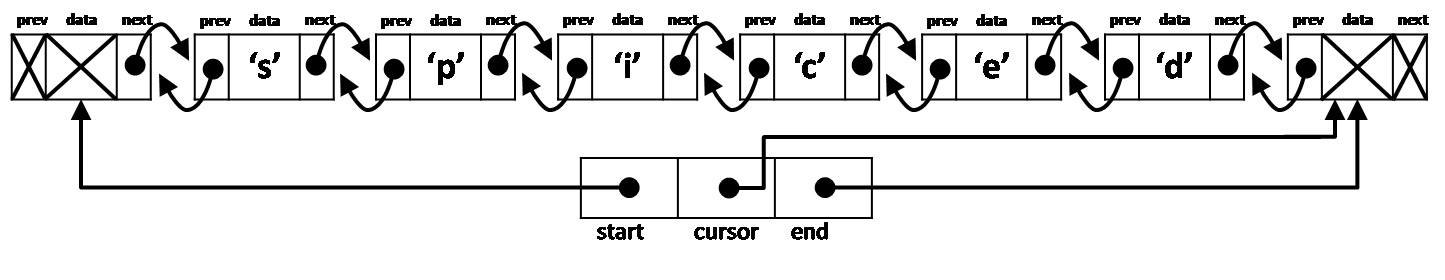
\includegraphics[width=0.95\textwidth]{\img/dll5.png}
\end{center}\vspace{-2.5ex}\enlargethispage{5ex}
A new, empty text buffer \lstinline'B' containing no text has a header and
two nodes and the cursor at the \lstinline'end':
\begin{center}
  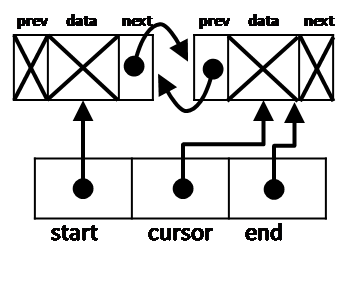
\includegraphics[width=0.23\textwidth]{\img/dll6.png}
\end{center}


\subsection{Data structure invariants}

We use doubly-linked lists to implement \emph{text buffers}, which
have type \lstinline'tbuf*'.
\begin{quote}
\begin{lstlisting}[numbers=none]
typedef struct tbuf_header tbuf;
struct tbuf_header {
    dll* start;
    dll* cursor;
    dll* end;
};
\end{lstlisting}
\end{quote}
A valid text buffer is a non-\lstinline'NULL' \lstinline'tbuf*' with the
following properties:
\begin{itemize}
        \item the \lstinline'next' links proceed from the
          \lstinline'start' node to the \lstinline'end' node, with the
          \lstinline'cursor' node included in the segment from
          \lstinline'start' (exclusive) to \lstinline'end' (inclusive).
  \item the \lstinline'prev' links mirror the \lstinline'next' links.
\end{itemize}
These are our \emph{linking invariants}.

\begin{task}[5]
\TAGS{ds-invariant, linked-list, pointer}
In the file \lstinline'tbuf.c0',
implement the function
\begin{quote}
\lstinline'bool is_tbuf(tbuf* B)'
\end{quote}

\noindent that formalizes the linking invariants on a doubly-linked
list text with a cursor.
\end{task}


You may find that writing a helper function
\lstinline'bool is_dll_segment(dll* a, dll* b)' will help you implement
\lstinline'is_tbuf'. You are not required to check for circularity, but
you may find it to be a useful exercise (it's actually easier for a
doubly linked list than for singly-linked ones).

This task is not trivial. There are many ways for a doubly-linked list
to be invalid, even without circularity. For instance, your
\lstinline'is_tbuf' function will be tested against structures with
\lstinline'NULL' pointers in various locations and against almost-correct
doubly-linked lists:

\bigskip

\enlargethispage{1ex}
\noindent
\begin{minipage}{0.55\linewidth}\centering
  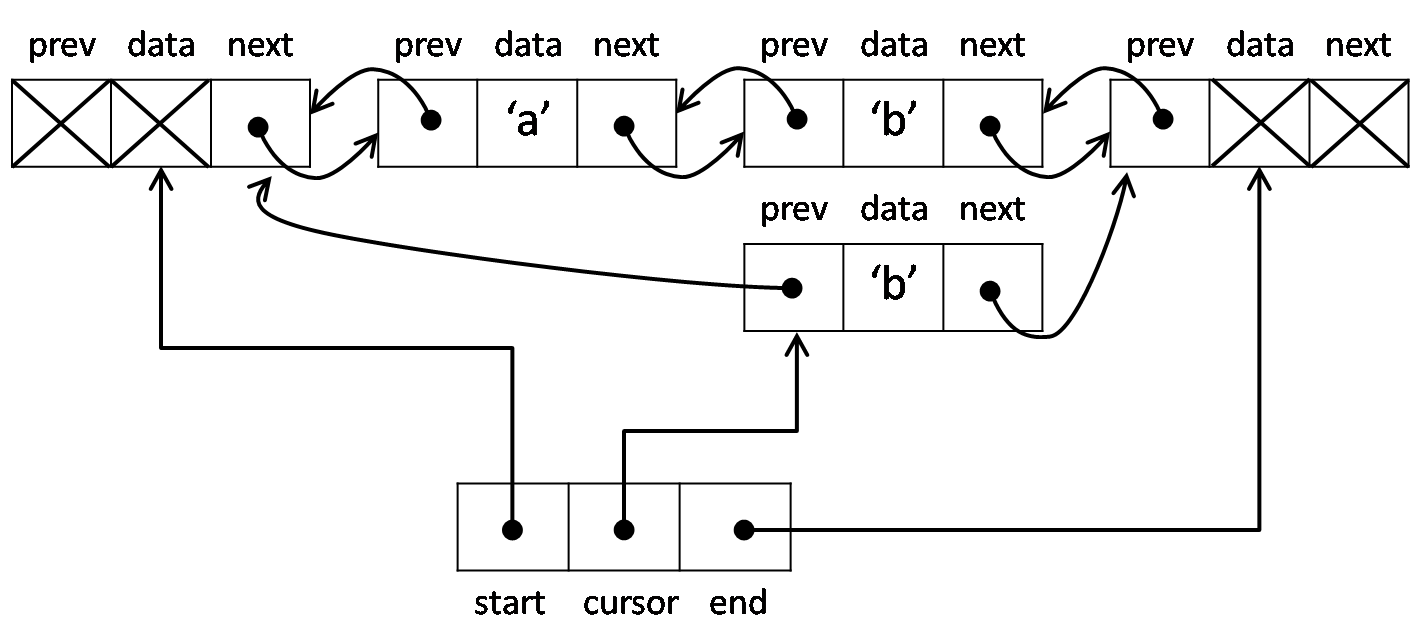
\includegraphics[width=0.95\textwidth]{\img/baddll2.png}
\end{minipage}\hspace{1em}
\begin{minipage}{0.35\linewidth}
  Not a doubly-linked list (the \lstinline'cursor' isn't on the path from
  \lstinline'start' to \lstinline'end').
\end{minipage}
\hfill

\vfill

\noindent
\begin{minipage}{0.55\linewidth}\centering
  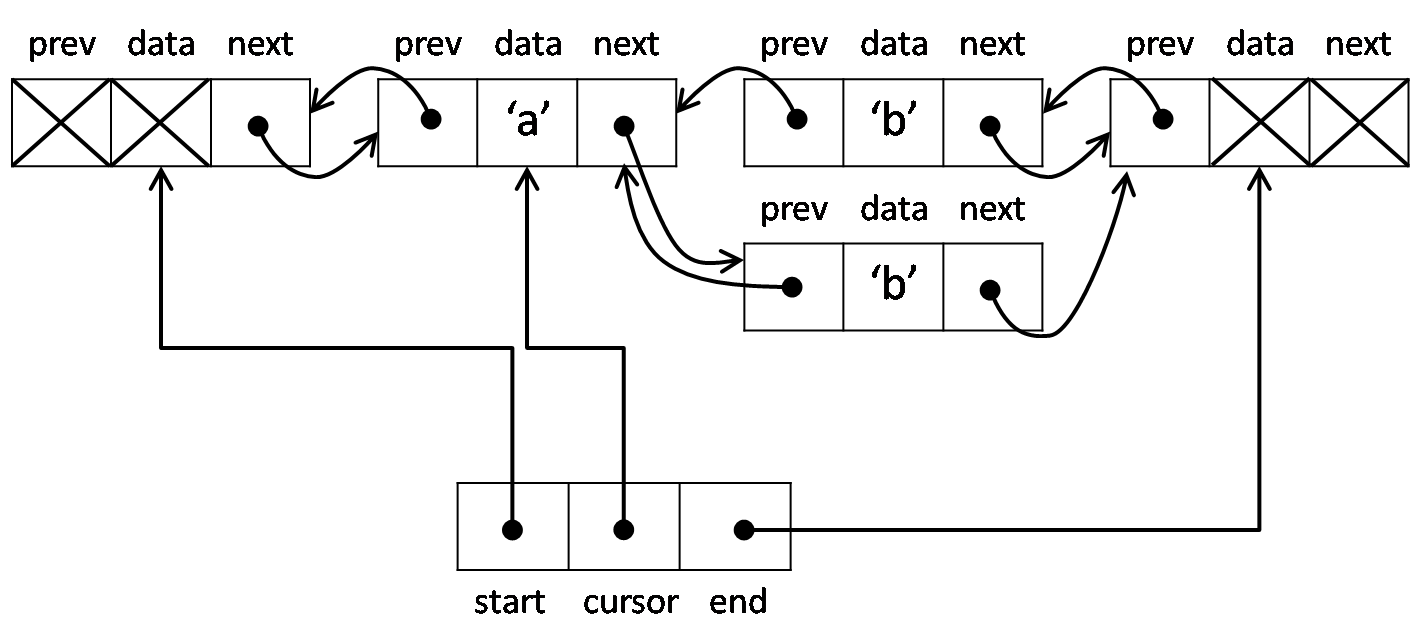
\includegraphics[width=0.95\textwidth]{\img/baddll3.png}
\end{minipage}\hspace{1em}
\begin{minipage}{0.35\linewidth}
  Not a doubly-linked list (the \lstinline'prev' links don't mirror the
  \lstinline'next' links).
\end{minipage}
\hfill

\clearpage
\subsection{Manipulating doubly-linked lists}

\begin{task}[9]
\TAGS{ds-invariant, linked-list, pointer}
Implement the following utility functions on doubly-linked lists with cursors:

\begin{quote}
\begin{tabular}{p{0.45\textwidth}p{.45\textwidth}}
    \textbf{Function:}             & \textbf{Returns true iff...} \\
    \lstinline"bool tbuf_at_left(tbuf* B)"
      & \ldots{t}he cursor is as far left as possible \\
    \lstinline"bool tbuf_at_right(tbuf* B)"
      & \ldots{t}he cursor is as far right as possible \\
\end{tabular}
\end{quote}

\noindent
and the following interface functions for manipulating doubly-linked
lists with cursors:

\begin{quote}
\begin{tabular}{p{0.45\textwidth}p{.45\textwidth}}
 \lstinline"tbuf* tbuf_new()" & Create a new and empty text buffer \\
 \lstinline"void tbuf_forward(tbuf* B)" & Move the cursor forward, to the right \\
 \lstinline"void tbuf_backward(tbuf* B)" & Move the cursor backward, to the left \\
 \lstinline"char tbuf_delete(tbuf* B)" & Remove the node to the cursor's left \\
 & (should return the deleted \lstinline'char') \\
 \lstinline"void tbuf_insert(tbuf* B, char c)" & Insert \lstinline'c' to the cursor's left \\
\end{tabular}
\end{quote}
\end{task}
\noindent
\textbf{If an operation cannot be performed, a contract
(precondition) should
fail.}
These functions should require and preserve the data structure
invariant you wrote above, and you should both document this fact and
use it to help write the code.

\subsection{Rows and columns}

Up until now, nothing that we've written has been specific to
doubly-linked lists of \emph{characters}. One thing we care a great
deal about in a text editor is which characters are newlines, because
that is what lets us know our position in the document: the row and
column. In Emacs, the first row is row 1, and the first column is
column 0. In these Emacs buffers, you can see the (row,
column) displayed in the lower right corner:
\begin{center}
  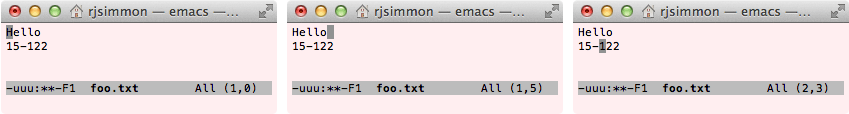
\includegraphics[width=\textwidth]{\img/emacs-rowcol.png}
\end{center}

We can calculate the column of the cursor by working backwards until
we find a newline, and we can calculate the row of the cursor by
working backwards to the beginning of the buffer and counting the
newlines. Note that in the middle example, the cursor is atop a cell
containing a newline \lstinline"'\n'", but the cursor is at the end of
row 1, not the beginning of row 2.

\begin{task}[2]
\TAGS{ds-invariant, linked-list, pointer}
Implement the following functions on doubly-linked lists with cursors:

\begin{quote}
\begin{tabular}{p{0.45\textwidth}p{.45\textwidth}}
    \textbf{Function:}             & \textbf{} \\
    \lstinline"int tbuf_row(tbuf* B)"
      & Return the row of the cursor \\
    \lstinline"int tbuf_col(tbuf* B)"
      & Return the column of the cursor \\
\end{tabular}
\end{quote}
\end{task}

\noindent
These functions should be as efficient as possible, only scanning necessary
portions of the doubly-linked list.


\subsection{Testing}

You can test your doubly-linked-list implementation interactively by
compiling and running the provided \lstinline'tbuf-test.c0', which
treats elements as C0~characters as in the illustration
above. You are encouraged to use this file as a starting point for
writing your own unit tests.
\begin{quote}
\begin{lstlisting}[language={[coin]C}]
% cc0 -d -w -o tbuf-test tbuf.c0 tbuf-test.c0 test-main.c0
% ./tbuf-test
Visualizing an initially-empty text buffer.
The '<' character mimics going backwards (left arrow key)
The '>' character mimics going forwards (right arrow key)
The '^' character mimics deletion (delete key)
The '@' character mimics a newline (enter key)
All other characters just insert that character

Give initial input (empty line quits):
\end{lstlisting}
\end{quote}
Suggestion: try entering ``\lstinline'steady^<<<<^>>^>>^@<<@^^'''
the initial input.


\clearpage
\section{Editor}

One desirable feature of a text editor is the ability to report the
current row and column. (You can display this information in Emacs by
typing ``\lstinline'M-x line-number-mode''' and
``\lstinline'M-x column-number-mode'''.)
In this section, we'll introduce
an \lstinline'editor' type which keeps track of both the cursor and the row
and column position.

\paragraph{Remember:}

You've already implemented your code for doubly-linked lists with
cursors, and hopefully you've tested that implementation
extensively. Avoid re-implementing features in this part of the
assignment! Whenever possible, reuse the functions you've already
implemented.

\subsection{Data structure invariants}
An editor keeps track of both the text buffer and \lstinline'int'
fields storing the row and column.

\begin{quote}
\begin{lstlisting}
typedef struct editor_header editor;
struct editor_header {
    tbuf* buffer;
    int row;
    int col;
};
\end{lstlisting}
\end{quote}
A valid editor data structure is non-\lstinline'NULL', has a valid
text buffer, and has recorded \lstinline'row' and \lstinline'col'
fields that match the information returned by the \lstinline'tbuf_row'
and the \lstinline'tbuf_col' functions.

\begin{task}[3]
\TAGS{ds-invariant, linked-list}
In the file \lstinline'editor.c0', implement the function
\begin{quote}
\lstinline'bool is_editor(editor* E)'
\end{quote}
\noindent that formalizes the data structure invariants on an editor.
\end{task}

\subsection{Manipulating text in the editor}

By tracking the row and column in the data structure, we can report
this information to the user without ever having to recalculate the
row using \lstinline'tbuf_row'. It's good to avoid this, because
\lstinline'tbuf_row' can be expensive to run. We will sometimes, but
only rarely, need to recalculate the column by calling
\lstinline'tbuf_col'. Any single row is usually relatively short (80
columns maximum, if you're using good style), so this should be fast.

Specifically, we only need to recalculate the column by calling
\lstinline'tbuf_col' when we delete a newline character or move left
from the beginning of one line to the end of the previous line.

\clearpage
\begin{task}[6]
\TAGS{application, ds-invariant, linked-list}
Efficiently implement the following interface functions for
manipulating editors:

\begin{quote}
\begin{tabular}{p{0.5\textwidth}p{.45\textwidth}}
 \lstinline"editor* editor_new()" & Create a new and empty editor \\
 \lstinline"void editor_forward(editor* E)" & Move the cursor forward, to the right \\
 \lstinline"void editor_backward(editor* E)" & Move the cursor backward, to the left \\
 \lstinline"void editor_delete(editor* E)" & Remove the node to the cursor's left \\
 \lstinline"void editor_insert(editor* E, char c)" & Insert \lstinline'c' to the cursor's left \\
\end{tabular}
\end{quote}
\end{task}
\textbf{These functions directly respond to a user's input.}  That
means that if an operation cannot be performed (e.g., pressing the
``left'' key to move the cursor backward with
\lstinline'editor_backward' when it's already at the left end), the
function should leave the text buffer \textbf{unchanged} instead of
raising an error or assertion violation.


\subsection{Testing}

The same testing program you used for testing your \lstinline'tbuf' implementation can also be used for this part of the assignment:
\begin{quote}
\begin{lstlisting}[language={[coin]C}]
% cc0 -d -w -o editor-test tbuf.c0 editor.c0 editor-test.c0 test-main.c0
% ./editor-test
\end{lstlisting}
\end{quote}
You can additionally test your code with a visual
text editor designed by legendary former TA and instructor William Lovas:
\begin{quote}
\begin{lstlisting}[language={[coin]C}]
% cc0 -d -w -o E0 tbuf.c0 editor.c0 lovas-E0.c0
% ./E0
\end{lstlisting}
\end{quote}

\begin{ectask}
\TAGS{application, ds-invariant, linked-list}
The \lstinline'lovas-E0.c0' file has two functions,
\lstinline'editor_up' and \lstinline'editor_down'. If you comment out
these lines and implement the up and down functions in
\lstinline'editor.c0', you can move around the buffer more effectively.

The up and down keys should take you up or down a row unless you're on
the first or last row (respectively) already. If possible, this
operation should leave you on the same column as before.  This is not
possible when the row you've landed on has too few columns. In that
case, you should leave the cursor at the rightmost end of the row.
\end{ectask}

\end{document}